\documentclass[10pt]{article}

% amsmath package, useful for mathematical formulas
\usepackage{amsmath}
% amssymb package, useful for mathematical symbols
\usepackage{amssymb}

% graphicx package, useful for including eps and pdf graphics
% include graphics with the command \includegraphics
\usepackage{graphicx}

% cite package, to clean up citations in the main text. Do not remove.
\usepackage{cite}

\usepackage{color} 

% Use doublespacing - comment out for single spacing
\usepackage{setspace} 
\doublespacing

% Text layout
\topmargin 0.0cm
\oddsidemargin 0.5cm
\evensidemargin 0.5cm
\textwidth 16cm 
\textheight 21cm

% Bold the 'Figure #' in the caption and separate it with a period
% Captions will be left justified
\usepackage[labelfont=bf,labelsep=period,justification=raggedright]{caption}

% Use the PLoS provided bibtex style
\bibliographystyle{plos2009}

% Remove brackets from numbering in List of References
\makeatletter
\renewcommand{\@biblabel}[1]{\quad#1.}
\makeatother


% Leave date blank
\date{}

\pagestyle{myheadings}
%% ** EDIT HERE **

\usepackage{multirow}

%% ** EDIT HERE **
%% PLEASE INCLUDE ALL MACROS BELOW

% figure files reside in the figures/ directory
\graphicspath{
{figures/}
}

%% END MACROS SECTION

\begin{document}

% Title must be 150 characters or less
\begin{flushleft}
{\Large
\textbf{Spatially explicit model of the lymphocyte diaspora in influenza-infected lung quantifies constraints of chemokine directed migration (SUPPLEMENT)}
}
% Insert Author names, affiliations and corresponding author email.
\\
Drew Levin$^{1,\ast}$, 
Stephanie Forrest$^{1}$, 
Soumya Banerjee$^{1}$
Candice Clay$^{2}$, 
Melanie Moses$^{1}$, 
Frederick Koster$^{1,2}$, 
\\
\bf{1} Department of Computer Science, University of New Mexico, Albuquerque, NM, USA
\\
\bf{2} Lovelace Respiratory Research Institute, Albuquerque, NM, USA
\\
$\ast$ E-mail: Corresponding drew@cs.unm.edu
\end{flushleft}


% You may title this section "Methods" or "Models". 
% "Models" is not a valid title for PLoS ONE authors. However, PLoS ONE
% authors may use "Analysis" 
\section{Models}

\subsection{Delay Differential Equation Model}

We adapt the delay differential equations first presented in \cite{Mitchell2011} to find values for chemokine production rates.  We use initial populations and parameter values from the previous study while adding an extra equation to model chemokine production (final equation):

\begin{equation*}
\label{EqS1}
\begin{aligned}
\dot{T} &= - \beta T V \\
\dot{I_1} &= \beta T V - \beta T[t-\tau_1]V[t-\tau_1] \\
\dot{I_2} &= \beta T[t-\tau_1]V[t-\tau_1] - \delta I_2 \\
\dot{V} &= \frac{p}{1+eF} I_2  - \beta T V  \\
\dot{F} &=  I_1[t-\tau_2] \\
\dot{C} &= r I[t-\tau_3] - d C \\
\end{aligned}
\tag{\textbf{S}1}
\end{equation*}
\vspace{.05in}

$C$ represents the chemokine population.  Two parameters, $r$ and $d$, control the rate of chemokine production and the rate of chemokine decay.  Chemokine decay, $d$, was set to $3.8508\cdot10^{-4}$/s, which equates to a 30 minute half-life. $r$, being the only free parameter, was fit to the empirical data shown in Fig. 1 of the main paper using Matlab's \texttt{nlinfit} function.  This process was repeated six times, once for each set of data.  $\tau_3$, the chemokine production delay, was set to 8 hours for IP-10 fits and 16 hours for RANTES fits.

\subsection{T Cell Production Rate}

To find a value for $\sigma$ we use a differential equation model from \cite{Miao20101}:

\begin{equation*}
\label{EqS2}
\begin{aligned}
\dot{N_{c}} &= \sigma - \frac{r'^{2} \cdot N_{c}}{R^{2} \cdot t_{rc}}    & \pi r'^{2} &= a \sqrt{I} + b \\
\dot{N'_{f}} &= \frac{(r'^{2} - r^{2}) \cdot N_{c}}{R^{2} \cdot t_{rc}} - \frac{v_{tcell}}{(r' - r) / 2} \hspace*{2cm}  & \pi r^{2} &= \pi r_{cell}^{2} \cdot I \\
\dot{N_{f}} &= \frac{r^{2} \cdot N_{c}}{R^{2} \cdot t_{rc}} + \frac{v_{tcell}}{(r' - r) / 2} \\
\dot{T} &= \rho T -\beta TV \\
\dot{I} &= \beta TV - \delta I - k_{e} N_{f} I \\
\dot{V} &= pI - \beta TV - \gamma (t) V \\
\gamma (t) &= \left\{ \begin{array}{rcl}
	1/\mbox{day} & \mbox{,}  & t < 5  \\
	3/\mbox{day} & \mbox{,} & t \geq 5  
	\end{array}\right. \\
\end{aligned}
\tag{\textbf{S}2}
\end{equation*}
\vspace{.05in}

where $N_{c}$ is the number of circulating activated antigen-specific T cells, $N'_{f}$ is the number of circulating T cells that have found and exit into a region of lung tissue expressing chemokines and $N_{f}$ is the number of circulating T cells that have found an infected region. $T$ is the number of uninfected target cells, $I$ is the number of productively infected cells, and $V$ is the viral titer in serum. The infected region is assumed to be of radius $r$ and is within a region expressing chemokines of radius $r'$ ($r  < r'$). The lung is assumed to be a circular region with radius $R$. The area of the infected region is equal to the area of an infected cell (of radius $r_{cell}$) multiplied by the number of infected cells. The area of the region expressing chemokine was found to be related non-linearly to the number of infected cells ($\pi r'^{2} = a \sqrt{I} + b$) where $a$ and $b$ are constants that depend on the viral strain.

Circulating activated antigen-specific T cells ($N_{c}$) are assumed to be released from lymph nodes at a constant rate $\sigma$. These circulating cells then transition into $N'_{f}$ and $N_{f}$ at rates proportional to the areas of the chemokine expressing and infected regions relative to the whole lung area. Circulating cells that are in the chemokine expressing region ($N'_{f}$) transition to the infected region after walking randomly for an average time proportional to the difference in the radii between the two regions ($r' - r$). Target cells ($T$) become infected by virus at rate $\beta TV$, where $\beta$ is the rate constant characterizing infection. Infected cells ($I$) die at rate $\delta$ in addition to being lysed by T cells ($N_{f}$) at a rate $k_{e}$. Finally the viral titers ($V$) increase due to production of virus at rate $p$ by infected cells. Virus is also cleared due to uptake by infected cells (at a rate $- \beta TV$) and due to antibody (at a rate $\gamma (t)$ that changes after 5 days post infection). The initial viral titer was initialized to 10,000 PFUs and the initial number of target cells was one million. The initial number of infected cells is assumed to be zero. This ODE was fit to data taken from \cite{Miao2010} using Matlab's \texttt{nlinfit} function in order to obtain a value for $\sigma$.

% Results and Discussion can be combined.
\section{Results}

\subsection{Stochastic modeling effects}

Unlike ODE models, which are deterministic, stochastic models such as CyCells can produce different results on different runs (Figure~\ref{fig:variance}).  To test the strength of this effect, we ran each model fifty times using the default parameters given in Table~\ref{table:parameters}.  $R^2$ values were calculated for individual runs versus the average of all runs.  Pandemic H1N1 showed the least inter-run variance with an mean $R^2$ value of 0.9935 and standard deviation of 0.0029.  sH1N1 had a mean $R^2$ 0.9859 with a standard deviation of 0.0109.  aH5N1 had a mean $R^2$ of 0.9167 with a standard deviation of 0.0726.  

Each run took the calculated viral production and chemokine production rates for the three different strains of influenza as input and reported the total number of infected cells, including incubating, virus secreting and apoptotic, but not including dead cells.  Therefore the figures approximate plaque growth over time.

Overlaying multiple runs on a single plot reveals a slight growth rate transition 3 days p.i., which reflects the addition of IgM.  In addition, for each infection the number of infected cells declines quickly at day five due to the T cell response. 

The three strains show different levels of virulence, consistent with the results found in \cite{Mitchell2011} (Fig.~\ref{fig:variance}).  The rapid production of the pandemic H1N1 virus prevents the immune response from containing the infection.  Because pH1N1 is replicates at such a rapid rate, the window of opportunity for T Cells to gain ground is too small.  aH5N1 is cleared completely, sH1N1 is contained but not fully cleared, and pH5N1 recovers and continues to expand.



\subsection{Chemokine combinations}

Because aH5N1 has been shown to suppress the production of interferon \cite{Mitchell2011}, we hypothesize that it renders IP-10 ineffectual.  We hypothesize that this leads to the elevated RANTES secretion rates measured in aH5N1 compared to the other two strains (Table~\ref{table:strains}).  Because of this behavior IP-10 was not included in the aH5N1 model runs.  Four models runs were performed for each strain (two for aH5N1) to look at how the presence and/or lack of specific chemokines affect the simulated immune response (Fig.~\ref{fig:chemokine}).  The lack of both chemokines leads to runaway infections in all three strains.  The presence of only RANTES is enough to contain the aH5N1 infection, but is weaker than IP-10 in both H1N1 strains.  IP-10 alone proves to be as effective as the combination of IP-10 and RANTES, suggesting that RANTES does not play a significant role in infections that stimulate an IP-10 response.  We assume receptor sensitivity is the same for both chemokines and that the chemokines in combination work additively.


% The bibtex filename
\bibliography{references}

\section*{Figure Legends}

%\begin{figure}[!ht]
%\begin{center}
%%\includegraphics[width=4in]{figure_name.2.eps}
%\end{center}
%\caption{
%{\bf Bold the first sentence.}  Rest of figure 2  caption.  Caption 
%should be left justified, as specified by the options to the caption 
%package.
%}
%\label{Figure_label}
%\end{figure}


\begin{figure}[ht!]
\begin{center}
 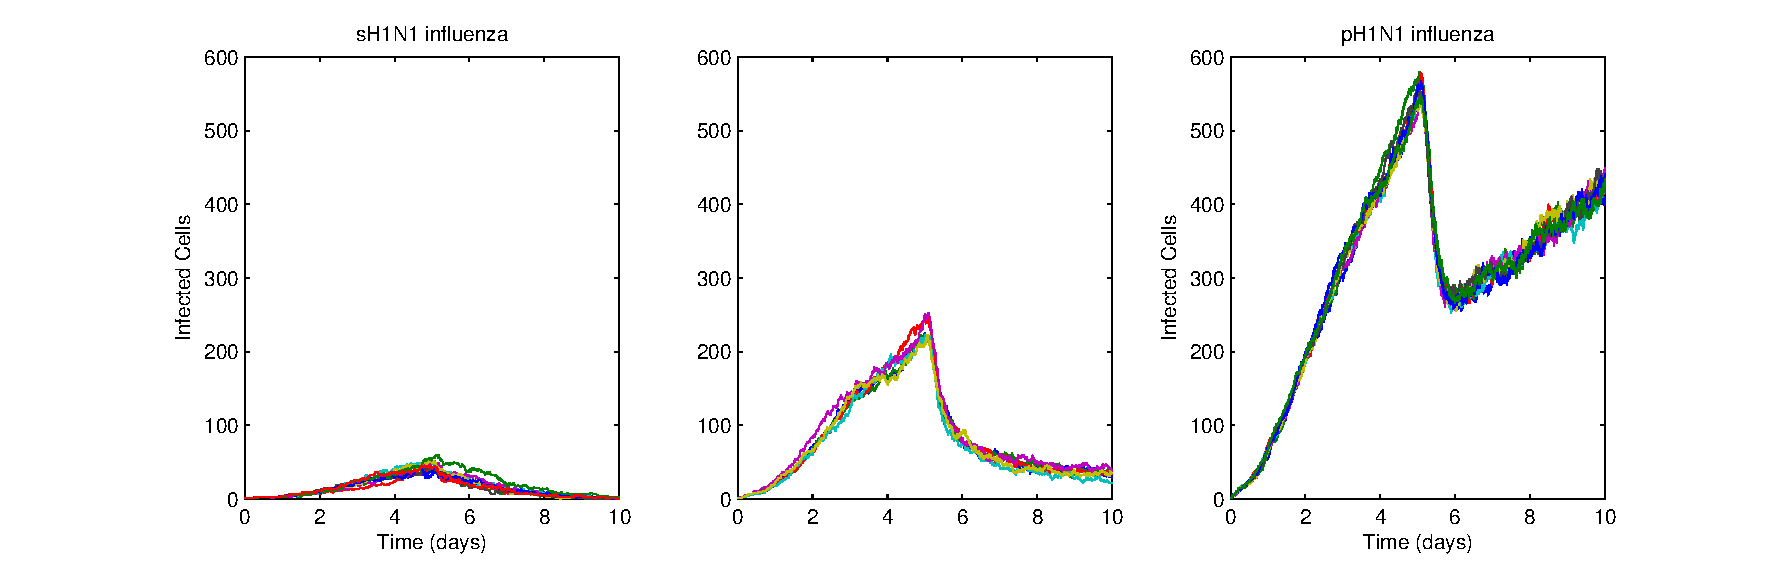
\includegraphics[width=\textwidth]{variance}
 \end{center}
\caption{Model results: Time series plots of fifty runs of aH5N1 (A), sH1N1 (B), and pH1N1 (C) infections (gray). IP-10 and RANTES were simulated in each run, except for aH5N1, which  produced only RANTES.  Each run was initialized identically for each strain save for the random seed.  The middle line shows the average while the outer lines show the 95\% confidence interval.} 
 \label{fig:variance}
\end{figure}


\begin{figure}[ht!]
\begin{center}
	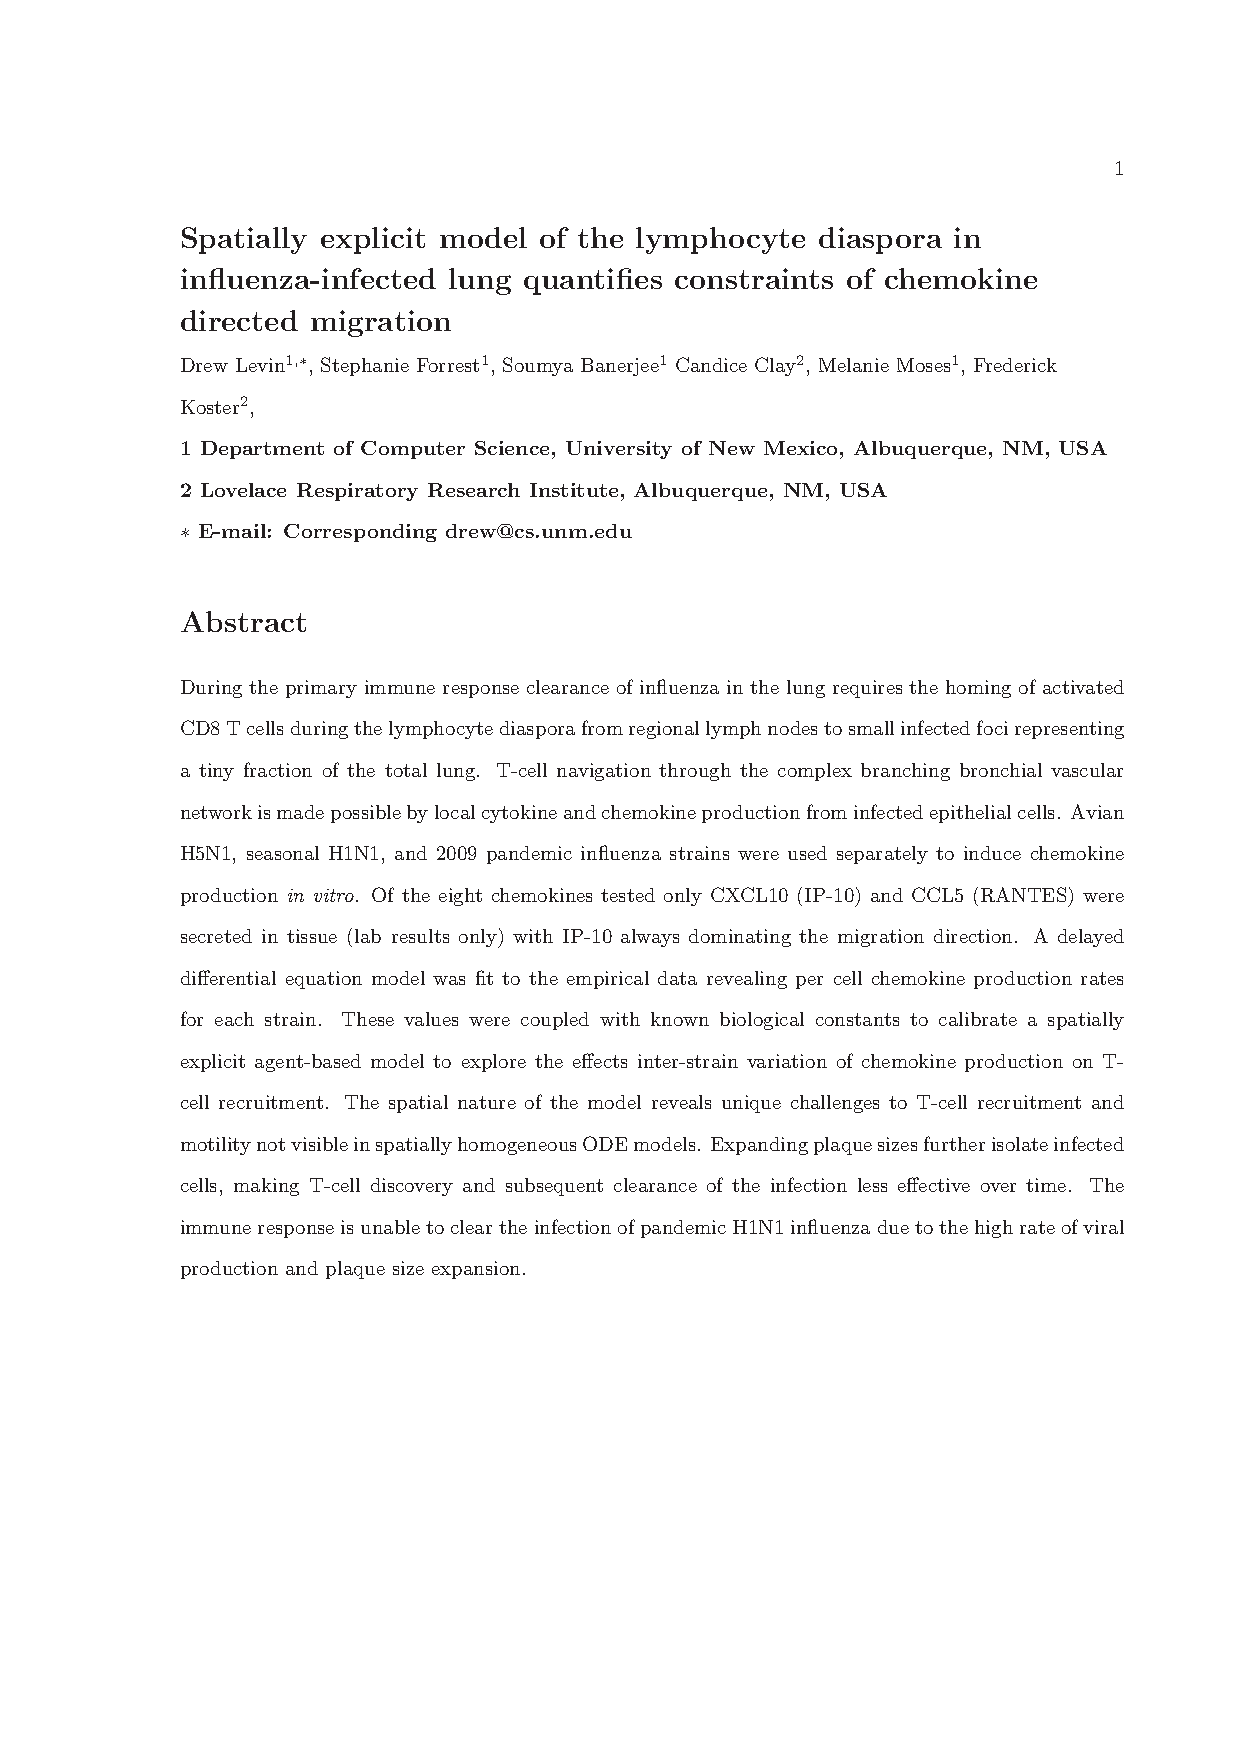
\includegraphics[width=\textwidth]{chemokine}
	\caption{Effects of different chemokine combinations.  A) aH5N1 does not stimulate an IP-10 response.  B-C) sH1N1 and pH1N1 show no significant difference between IP-10 alone versus IP-10 and RANTES combined.}
	\label{fig:chemokine}
\end{center}
\end{figure}

\section*{Tables}

%\begin{table}[!ht]
%\caption{
%\bf{Table title}}
%\begin{tabular}{|c|c|c|}
%table information
%\end{tabular}
%\begin{flushleft}Table caption
%\end{flushleft}
%\label{tab:label}
% \end{table}

\begin{table}[!ht]
\begin{center}
\begin{tabular}{ | c | c | c | }
  \hline                        
  Paramter & Value & Source \\
  \hline
  T(0) & $1e6$ & \cite{Mitchell2011} \\
  V(0) &  $1e4$ & \cite{Mitchell2011} \\
  $r_{cell}$ &  $10 \mu m$ & \cite{Miao2010} \\
  $t_{rc}$ & $6s$ & \cite{Peters1983} \\
  $v_{tcell}$ & $0.3 \mu m/s$ & \cite{Miller2003} \\
  $k_e$ & $6.4e-5/cell/day$ & \cite{Miao2010} \\
  $\beta$ & $4.8e-7/cell/PFU$ & \cite{Mitchell2011} \\
  $p$ & $0.18 PFU/h$ & \cite{Mitchell2011} \\
  $\delta$ & $16.7 hours$ & \cite{Mitchell2011} \\
  $a$ & $20.9$ & ABM fits \\
  $b$ & $70.8$ & ABM fits \\
  \hline  
\end{tabular}
\caption{Supplemental model parameters.  Most values are chosen to match the equations borrowed from both \cite{Mitchell2011} and \cite{Miao2010}.  Values \textit{a} and \textit{b} were fit to multiple runs of a simplified CyCells ABM.}
\label{table:supplement}
\end{center}
\end{table}

\end{document}
